\chapter{DUNE and the Far Detector}
\label{chapter:dune_fd}

%\noindent
The Deep Underground Neutrino Experiment (DUNE) \cite{DUNE2020TDR1} will consist of two neutrino detectors. A near detector complex will be placed in Fermilab, near Chicago, whereas a larger far detector will be built in the Sandford Underground Research Facility (SURF), South Dakota, approximately 1300 km away. It will address several questions in neutrino physics, study neutrinos from supernovae explosions and search for proton decay.

The liquid Argon time projection chamber (LArTPC) technology has been chosen for the far detector (FD) modules of DUNE. This experiment will record neutrino interactions from an accelerator-produced beam (the LBNF multi-megawatt wide-band neutrino beam planned for Fermilab) arriving at predictable times, but also aim at recording rare events such as supernova neutrinos or potential nucleon decays, requiring trigger schemes which can deal with both, and maximum uptime.

The neutrino beam to be used in DUNE will be provided by the LBNF beamline. First, an intense proton beam is extracted from the Fermilab Main Injector. Then, these protons with energies between $60 \ \mathrm{GeV}$ and $120 \ \mathrm{GeV}$ collide with a high-power production target and produce charged mesons. Two magnetic horns allow to focus the mesons and perform a sign selection (thus having the capability to switch between neutrino and antineutrino mode). Soon after that, the mesons decay and produce neutrinos (or antineutrinos) which are then aimed to SURF.

The aim of this Chapter is to review the main goals of the DUNE experiment, the design of the FD modules, the crucial role that the data acquisition (DAQ) system plays in the physics program of DUNE and the need for a ND.

\section{Physics goals of DUNE}

\begin{figure}[t]
	\centering
	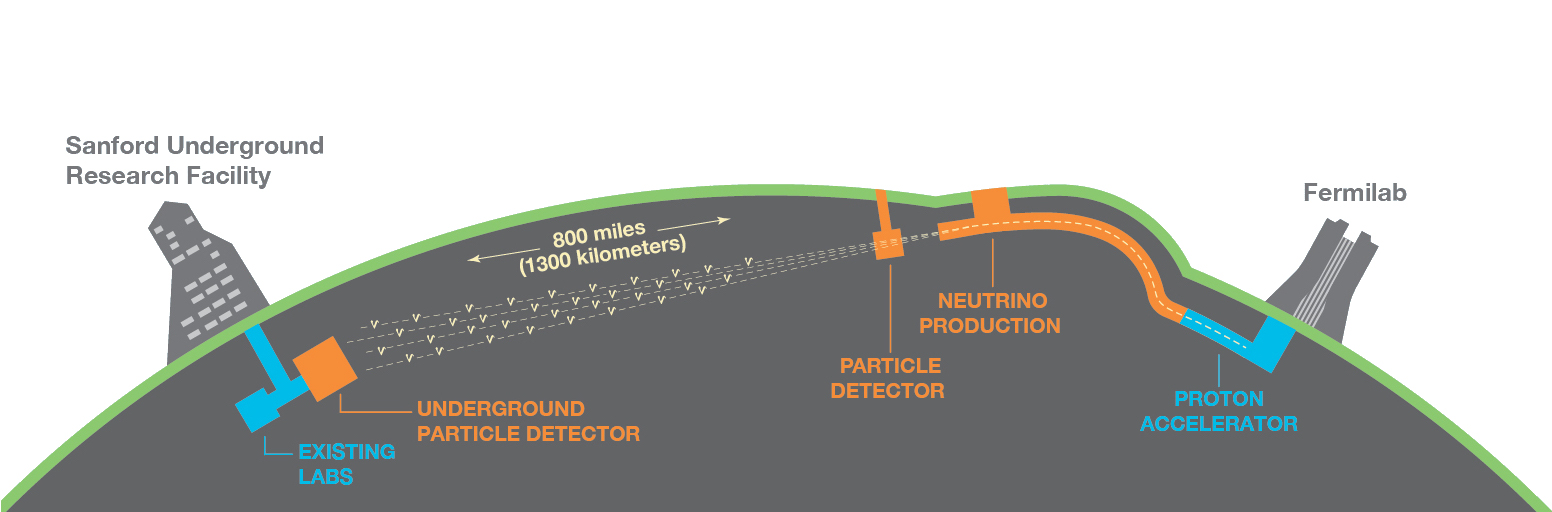
\includegraphics[width=0.9\linewidth]{Images/DUNE/FD/dune}
	\caption{Schematic diagram of the DUNE experiment \cite{DUNE2020TDR}.}
	\label{fig:dune}
\end{figure}

As noted in the literature (see for instance Ref. \cite{deSalas2020} for a review), the parameter space of the neutrino oscillation phenomena within the three-flavour picture is quite constrained by current experimental data. However, there are still crucial open questions, like the mass ordering and the value of $\delta_{CP}$. One of the main goals of DUNE is to shed some light on the values of these parameters \cite{DUNE2020TDR2}.

To address these questions DUNE can look to the subdominant oscillation channel $\nu_{\mu} \rightarrow \nu_{e}$ ($\bar{\nu}_{\mu} \rightarrow \bar{\nu}_{e}$) and study the energy dependence of the $\nu_{e}$ ($\bar{\nu}_{e}$) appearance probability. When we focus on the antineutrino channel $\bar{\nu}_{\mu} \rightarrow \bar{\nu}_{e}$ there is a change in the sign of $\delta_{CP}$, thus introducing CP-violation. Moreover, due to the fact that there are no positrons in the composition of Earth, there is a sign difference for the matter effect contribution when looking to the antineutrino channel. This asymmetry is proportional to the baseline length $L$ and is sensitive to the sign of $\Delta_{31}$, and thus to the neutrino mass ordering.

Another of the main physics goals of DUNE is the search for baryon-number violating (BNV) processes. Specifically, it will try to answer the question of whether protons are stable or not. There is no symmetry argument that forbids protons from decaying, but its apparent stability seems to suggest that baryon number is conserved \cite{Super-Kamiokande2009}. However, proton decay is a usual feature of grand-unified theories (GUTs), where electromagnetic, weak and strong interactions are unified above a certain energy scale \cite{Raby2006}.

As the energy deposition scale for this kind of searches is nearly the same as the one for long-baseline neutrino oscillations, DUNE will be able to look for them. It has several advantages over other experiments, such as excellent imaging and particle identification, which can be translated to lower backgrounds.

The last of the main objectives of DUNE is the detection of neutrinos originated in supernovae explosions, what is called a supernova neutrino burst (SNB). These neutrinos carry with them information about the core-collapse process, from the progenitor to the explosion and the remnant; but also may have information about new exotic physics. So far, the only neutrino events ever recorded from such a process were a few dozens of $\bar{\nu}_{e}$ events from the 1987A supernova located in the Magellanic Cloud, $50 \ \mathrm{kpc}$ away from Earth \cite{Kamiokande-II1987, Bionta1987}.

DUNE aims to collect also some SNB events. Despite these are quite rare, as the expected supernovae explosion events are about one every few decades for our galaxy and Andromeda, the long lifetime of the experiment (around a few decades as well) makes it reasonable to expect some. Nowadays the main sensitivity to SNB of most experiments is to the $\bar{\nu}_{e}$ through inverse beta decay. One of the advantages of DUNE is its expected sensitivity to $\nu_{e}$, since the dominant channel will be $\nu_{e}$ CC scattering.

Moreover, due to the stringent requirements that the main Physics goals set for DUNE, it will allow also to perform searches for all kind of BSM Physics. Among others, DUNE will be able to look for: active-sterile neutrino mixing, non-unitarity of the PMNS matrix, non-standard interactions, Lorentz and CPT violations, neutrino trident production, light-mass DM, boosted DM or heavy neutral leptons. In particular, the focus of my thesis will be the indirect DM searches at DUNE.

\section{}

\section{Far Detector}

\begin{figure}[t]
	\centering
	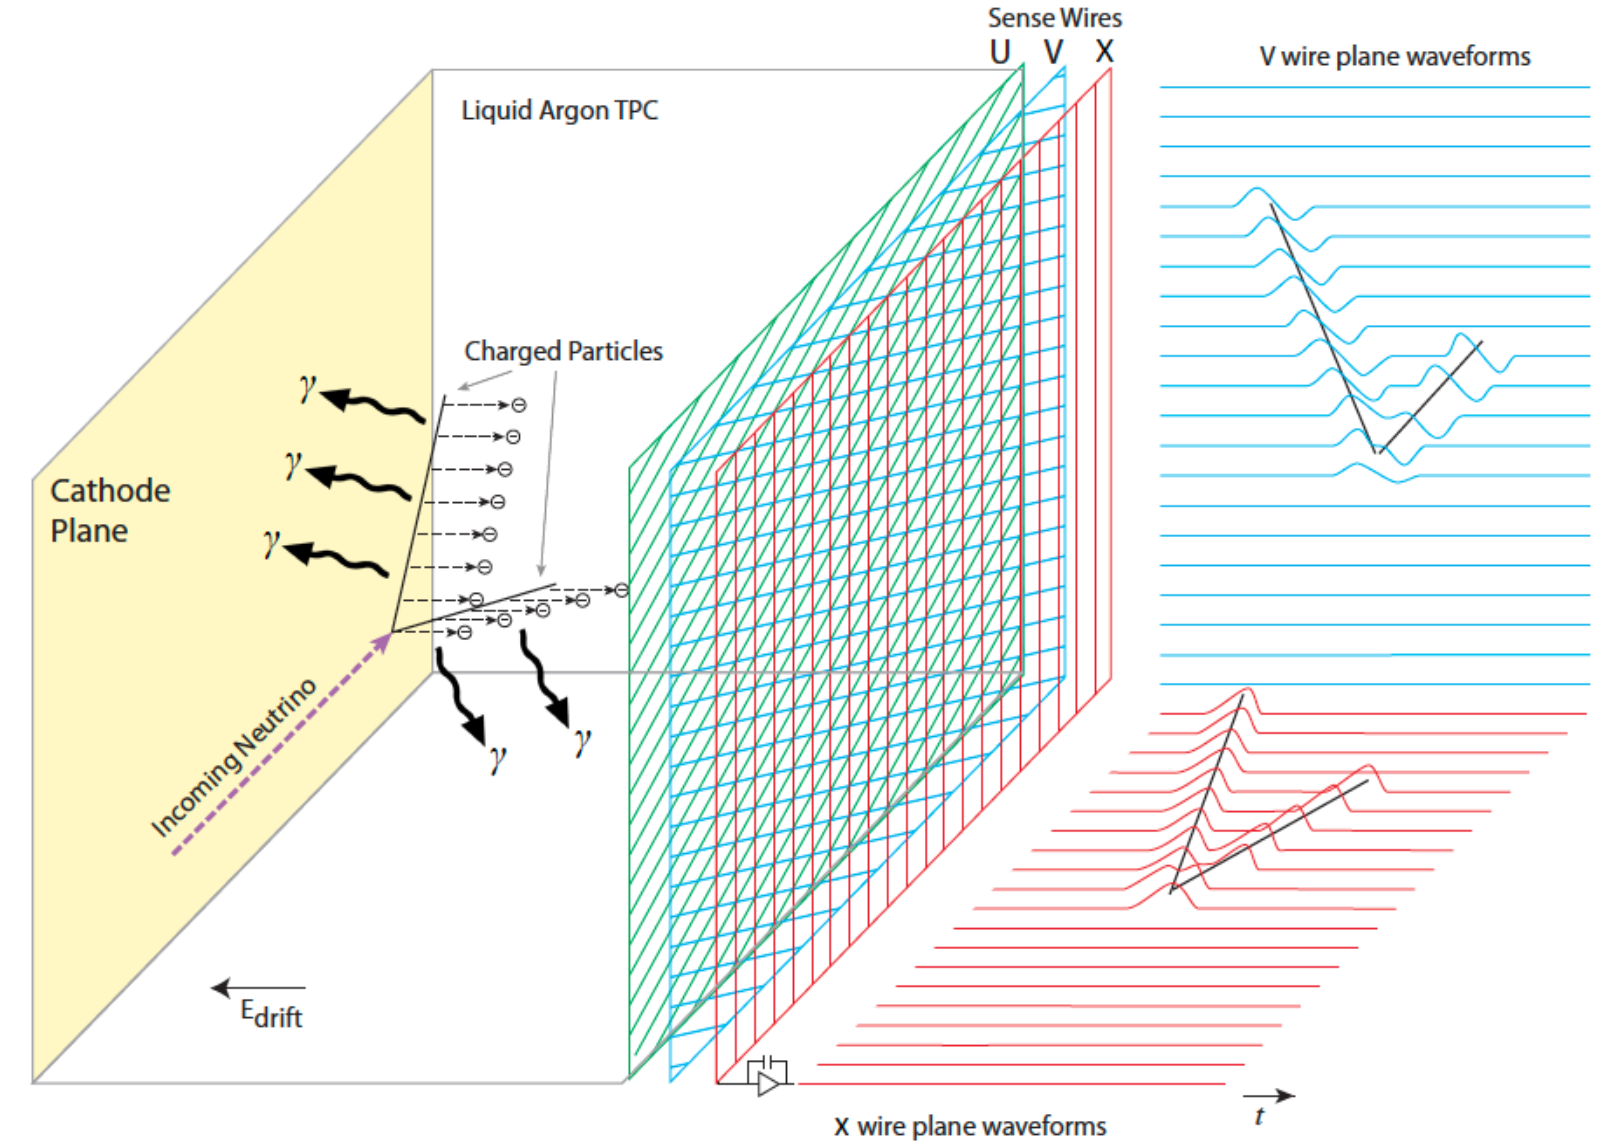
\includegraphics[width=0.8\linewidth]{Images/DUNE/FD/tpc}
	\caption{Schematic diagram showing the operating principle of a HD LArTPC.}
	\label{fig:tpc}
\end{figure}

The so-called DUNE Far Detector (FD) will consist on four liquid Argon (LAr) time projection chamber (TPC) modules with a LAr fiducial mass of at least $10 \ \mathrm{kt}$ each. These TPC modules are embedded in a cryostat of dimensions $15.1 \ \mathrm{m} \ (\text{w}) \times 14.0 \ \mathrm{m} \ (\text{h}) \times 62.0 \ \mathrm{m} \ (\text{l})$, located $1.5 \ \mathrm{km}$ underground at SURF. Nowadays there are two leading technologies for the design of the FD LArTPC modules:
\begin{itemize}
	\item Horizontal drift (HD): where the ionisation electrons produced as charged particles traverse the LAr drift horizontally towards the anode planes, made out of three layers of wire readout, due to the effect of an electric field. 
	\item Vertical drift (VD): where electrons will drift vertically until they meet a printed circuit board-based (PCB) readout plane. It is based on the original dual-phase (DP) design.
\end{itemize}
The HD design, previously known as single-phase (SP), was tested by the ProtoDUNE-SP detector at CERN. This prototype collected data from a hadron beam and cosmic rays, providing high-quality data sets for calibration studies and proving the excellent performance of this design. The other prototype deployed at CERN, known as ProtoDUNE-DP, used a vertical drift design with an additional amplification of the ionization electrons using a gaseous Argon layer above the liquid phase. Despite the advantage of signal gain, this design proved challenging to operate. The recently proposed VD design incorporates the positive features of both the ProtoDUNE-SP and ProtoDUNE-DP detectors.

For each event, with energies ranging from a few $\mathrm{MeV}$ to several $\mathrm{GeV}$, the detectors collect both the scintillation light and the ionization electrons produced by the interactions of charged particles in the liquid argon. In both designs the characteristic $128 \ \mathrm{nm}$ scintillation light of Argon produced is collected by a photon detection (PD) system. This light will indicate the time at which electrons start to drift, thus enabling reconstruction over the drift coordinate when compared to the time when the first electron arrives to the anode. Reconstruction of the topology in the traverse direction is achieved using the charge readout.

In the present report I am going to focus mainly on the HD technology, as an important part of the work is based on ProtoDUNE-SP data. Each HD detector module is divided in four drift regions, with a maximum drift length of $3.5 \ \mathrm{m}$ and a drift electric field of $500 \ \mathrm{V/cm}$. It features three anode planes built by stacking anode plane arrays (APAs), 2 high times 25 wide. Each APA is made of 2560 active wires, arranged in three layer, plus an extra grid layer. We have the collection or $X$ layer, followed by the two collection layers $V$ and $U$. The induction wires generate bipolar signals, negative when the drift electrons come to them and positive when they go drift far from the layers. The collection wires produce only a monopolar positive signal. The spacing between the wires is $\sim 5 \ \mathrm{mm}$, and it defines the spatial resolution of the APA.

The front-end readout electronics, or cold electronics (CE) as they are immerse in the LAr, are attached to the top of the up APAs and the bottom of the down APAs. Mounted in the front-end mother boards (FEMBs) we have a series of ASICs that digitize the signals from the collection and induction planes. Each wire signal goes to a charge-sensitive amplifier, then there is a pulse-shaping circuit and this is followed by the analogue-to-digital converter. This part of the process happens inside the LAr to minimise the number of cables penetrating the cryostat. The digitised signals come out finally via a series of high-speed serial links to the warm interface boards (WIBs), from where the data is sent to the back-end DAQ through optical fibers.

When using a SP LArTPC there is no electron amplification, thus low noise is required by CE to extract the signals from the wires with a minimum S/N. In the worst operating case (short drift electron lifetime $\tau = 3 \ \mathrm{ms}$ and $E_{drift} = 250 \ \mathrm{V/cm}$) at least $10^{4}$ electrons will arrive to the anode from a minimum ionizing particle (MIP) near the cathode (farthest possible distance). Requiring at most $10^{3}$ electrons of equivalent noise charge (ENC) we will have a S/N $~\sim10$ for the collection wires. In the induction wires it results in S/N $\sim 5$, because of the bipolar shape of the signal. Keeping noise low (improving S/N) is crucial to achieve the Physics goals. It allows proper event reconstruction and expand the boundaries on low-energy phenomena (SNB, $^{39}$Ar calibrations, etc.). Noise also affect DAQ bandwidth, and can be a problem for astrophysical measurements.

\section{Data Acquisition System}

The task of the data acquisition (DAQ) system is to receive, process and store data from the detector modules. In the case of DUNE the DAQ architecture is designed to work for all FD modules interchangeably, except some aspects of the upstream part which may depend on the specific module technology.

The enormous sample rate and the number of channels in TPC and PD readouts will produce a very large volume of data. These pose really strong requirements and challenges to the DUNE FD DAQ architecture. It will be required to read out data of the order of ten thousand or more channels at rates of a few MHz. In order to cope with the huge data volume, segmented readouts and compression algorithms are used to reduce the data rate to manageable levels. My work for the last months focused on the FD upstream DAQ. It receives raw data from detector, buffers it, and performs a portion of low-level data selection, the so-called Trigger Primitive (TP) generation.

The DAQ system of the DUNE FD is composed of five different subsystems. The first one is the upstream DAQ, which receives the raw data from the detector, buffers it and perform some low-level pre-processing. The details of this specific subsystem will be discussed in more detail in the following Sec. \ref{sec:5.1}. The minimally processed data is then fed into a hierarchical data selection (DS) system, which then performs a module level trigger decision. In case of a positive decision a trigger command is produced and executed by the data flow orchestrator (DFO), located in the back-end (BE) DAQ subsystem. Subsequently the DAQ BE retrieves the relevant data from the buffers located in the upstream DAQ, adds all the data into a cohesive record and saves it to permanent storage. Watching over all the other subsystems we also have the control, configuration and monitoring (CCM) subsystem and the time and synchronization subsystem. Fig. \ref{fig:daq1} shows a schematic diagram of the DAQ system, showing the different subsystems and their relations.

\begin{figure}[t]
	\centering
	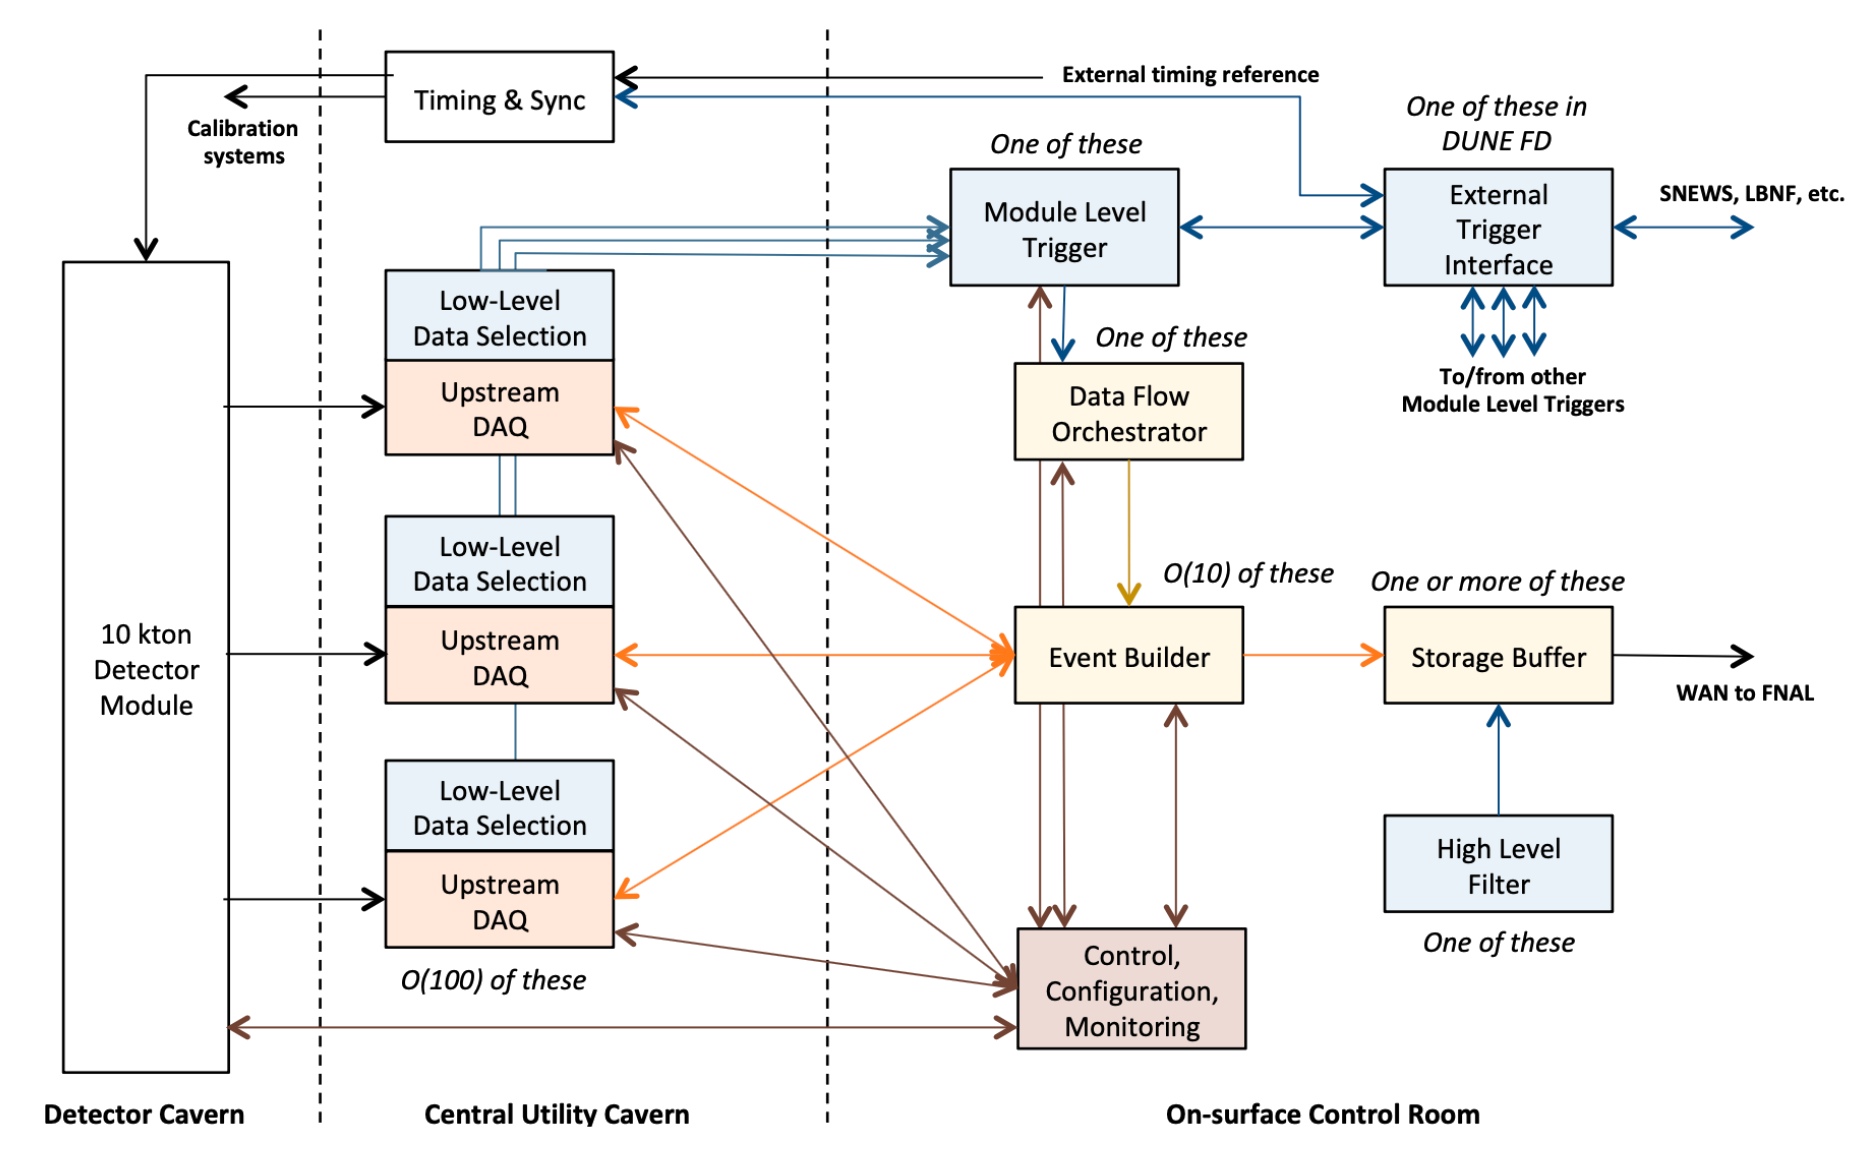
\includegraphics[width=0.8\linewidth]{Images/DUNE/FD/DAQ_detailed2}
	\caption{Detailed diagram of the FD DUNE DAQ system.}
	\label{fig:daq1}
\end{figure}

A notorious challenge for the DUNE DAQ system comes from the its broad physics goals. We must be prepared to process events spanning a wide range of time windows (from $5 \ \mathrm{ms}$ in the case of beam and cosmic neutrinos and nucleon decay to $100 \ \mathrm{s}$ in the case of SNBs) and therefore this requires a continuous readout of the detector modules. Moreover, because of the off-beam measurements we need to ensure the capabilities of online data processing and self-triggering. Having this into account, together with the technical constraints, the DUNE FD DAQ faces a series of challenges: it needs to be fault tolerant and redundant to reduce downtime, accommodate new components while it keeps serving the operational modules, have large upstream buffers to handle SNB physics, be able to support a wide range of readout windows and last reduce the throughput of data to permanent storage to be at most $30 \ \mathrm{PB/year}$.